%-----------------------------------------------------------------------------
%
%               Template for sigplanconf LaTeX Class
%
% Name:         sigplanconf-template.tex
%
% Purpose:      A template for sigplanconf.cls, which is a LaTeX 2e class
%               file for SIGPLAN conference proceedings.
%
% Guide:        Refer to "Author's Guide to the ACM SIGPLAN Class,"
%               sigplanconf-guide.pdf
%
% Author:       Paul C. Anagnostopoulos
%               Windfall Software
%               978 371-2316
%               paul@windfall.com
%
% Created:      15 February 2005
%
%-----------------------------------------------------------------------------


\documentclass{sigplanconf}
%\documentclass{sig-alternate}

% The following \documentclass options may be useful:

% preprint      Remove this option only once the paper is in final form.
% 10pt          To set in 10-point type instead of 9-point.
% 11pt          To set in 11-point type instead of 9-point.
% authoryear    To obtain author/year citation style instead of numeric.

\usepackage{ifthen}
\usepackage{color}
\usepackage{framed}
\usepackage{paralist}
\usepackage{mathtools}
\usepackage{alltt}
\usepackage{textcomp}
\usepackage{fixltx2e}
\usepackage{url}

\newboolean{td}
  \setboolean{td}{true} % modify here
  \ifthenelse{\boolean{td}}
             {\newcommand{\ph}[1]{\textcolor{blue}{PH: #1}}
               \newcommand{\lp}[1]{\textcolor{blue}{LP: #1}}
             }
             {\newcommand{\ph}[1]{}
               \newcommand{\lp}[1]{}
             }

\newenvironment{code}{\begin{alltt}\footnotesize}{\end{alltt}}
\newenvironment{smcode}{\begin{alltt}\scriptsize}{\end{alltt}}

%% \newenvironment{cols}{\begin{tabular}{m{3.6cm}|m{3.6cm}} &
%%     \\\hline}{\end{tabular}}

\newcommand{\cd}[1]{\texttt{#1}}

\begin{document}

\special{papersize=8.5in,11in}
\setlength{\pdfpageheight}{\paperheight}
\setlength{\pdfpagewidth}{\paperwidth}

\conferenceinfo{CONF 'yy}{Month d--d, 20yy, City, ST, Country} 
\copyrightyear{20yy} 
\copyrightdata{978-1-nnnn-nnnn-n/yy/mm} 
\doi{nnnnnnn.nnnnnnn}

% Uncomment one of the following two, if you are not going for the 
% traditional copyright transfer agreement.

%\exclusivelicense                % ACM gets exclusive license to publish, 
                                  % you retain copyright

%\permissiontopublish             % ACM gets nonexclusive license to publish
                                  % (paid open-access papers, 
                                  % short abstracts)

\titlebanner{banner above paper title}        % These are ignored unless
\preprintfooter{short description of paper}   % 'preprint' option specified.

\title{Embedded$^2$ Programming:\\Building Embedded Systems with Embedded DSLs}
\subtitle{(Experience Report)}

\authorinfo{You \and me \and everybody ...}
           {Galois, Inc.}
           {\{foo, bar, ...\}@galois.com}
%% \authorinfo{Name2\and Name3}
%%            {Affiliation2/3}
%%            {Email2/3}

\maketitle

\begin{abstract}
We describe our experience building two embedded domain-specific languages
hosted in Haskell for building large embedded systems and using them to build a
complex open-source autopilot, including device drivers, control laws, fail-safes,
and communication subsystem.
\end{abstract}

\category{CR-number}{subcategory}{third-level}

% general terms are not compulsory anymore,
% you may leave them out
%% \terms
%% term1, term2

\keywords
keyword1, keyword2

\section{Introduction}

Embedded programming involves the lowest levels of software development.  Most
development is in a low-level language, like C or assembly, and programs
interact intimately with the hardware directly.  Embedded domain-specific
languages (EDSLs) are in some sense at the other end of the software
spectrum: they are often embedded (in a different sense of the word!) in
high-level programming languages such as Haskell or ML, and are used to
lift the abstraction level for programmers.

While the abstraction levels are quite different, there is no in principle
reason why EDSLs cannot be used for embedded programming; this report is about
our experience in building new EDSLs for embedded programming and the benefits
and difficulties in using them.  Our experiences are based on synthesizing a
nearly 50 thousand lines of code (kloc) autopilot from our EDSLs.  The breadth
and scope of the project sets it apart.  The autopilot software is not just an
application, but a complete embedded system: SMACCMPilot's use of EDSLs includes
not just the core flight control algorithms, but also device drivers, encrypted
network stack, mode logic, and concurrency and task management.  It is one of
the largest (open-source) embedded systems projects developed using the EDSL
approach.

Our story is a largely positive one: we developed the languages and their (EDSL)
compilers from scratch in approximately \ph{XXX} engineer-months then we used
them to build SMACCMPilot in another \ph{YYY} engineer-months.  We achieved a
dramatic increase in productivity.  Furthermore, we achieved an increase in
code quality; our generated C code is free from memory-safety errors.

Our goal in this paper is to summarize some of our lessons-learned.  While we
use specific examples, the lessons apply more generally to industrially-large
embedded system design in EDSLs.  Our target audience includes both researchers
developing new EDSLs for low-level programming as well as practitioners
considering using EDSLs.


%% \lp{Indeed, a number of researchers have explored EDSLs for generating embedded
%%   C code, such as Atom~cite{}, Feldspar~\cite{}, Copilot~\cite{}, \lp{more}.
%%   However, these languages are still at the application level }

%% \lp{In this experience report, we describe lessons learned in the use of EDSLs to
%% build a complex embedded system: a secure autopilot called
%% \emph{SMACCMPilot}.\footnote{\emph{SMACCM} is an acronym for Secure
%%   Mathematically-Assured Composition of Control Models.}
%% }

\paragraph{Roadmap}
In Sections~\ref{sec:ivory} and~\ref{sec:tower}, we give a tour of the two EDSLs
we have developed in this project: Ivory, for synthesizing safe embedded C code,
and Tower, for synthesizing synchronous and asynchronous communicating
processes.  Using these languages, we have developed the SMACCMPilot autopilot,
described in Section~\ref{sec:smaccmpilot}.  We describe our more general
``lessons learned'' in Section~\ref{sec:thegood}, which apply generally to EDSLs
for embedded systems.


\section{Ivory: Safe C Programming}
\label{sec:ivory}

At face value, our approach sounds audacious if not ludicrous: faced with a
deadline for developing a new high-assurance autopilot system in one-and-a-half
years, start by designing a new programming language and compiler from the
ground up.

Of course, developing an EDSL is not the same as developing a stand-alone
compiler.  Much of the typical compiler tool-chain, such as the front-end
parser/lexer, is obviated.  Furthermore, we were confident that time spent in
writing the EDSL would be made up by developing in a high-level functional
language with a rich set of existing libraries. It took approximately 6
engineer-months to create the Ivory language and compiler, and total of about
6000 lines of Haskell code.

The language we developed for generating safe embedded C code is called
\emph{Ivory}.  Ivory shares the goal of other ``safe-C'' standalone languages
and compilers like Cyclone~\cite{cyclone} and Rust~\cite{rust}.  Our main
motivation for not using these languages is to have the benefits of an EDSL and
particularly our desire for a Turing-complete, type-safe macro-language to
improve our productivity.

There have also been some ``safe-C'' EDSLs including Atom~\cite{atom},
Copilot~\cite{copilot}, and FeldSpar~\cite{feldspar1}.  The most significant
difference between these languages and Ivory is that they are focused on pure
computations and do not provide convenient support for defining in-memory
data-structures and manipulating memory.  Ivory is designed to be a
general-purpose embedded C EDSL that can be used for memory-manipulation
intensive programs, such as device drivers.

The essential contributions of Ivory from a programming language perspective are
its expressiveness and our approach to type-safety.

\paragraph{Expressiveness}
Regarding the expressiveness, Ivory has a variety of useful features, including:
\begin{compactitem}
  \item \emph{Memory-areas}: the ability to allocate stack-based memory and
    manipulate both local and global memory areas~\cite{memareas}.
  \item \emph{Product types}: C structs with well-typed accessors.
  \item \emph{FFI}: typed interfaces for calling arbitrary C functions.
  %% \item \emph{Module system}: managing dependencies to support C-level headers
  %%   and includes.
  \item \emph{Bit-fields}: support for typed manipulation of bit-fields and
    registers~\cite{high-level}.
\end{compactitem}

As well, Ivory has some limitations, motivated by making analysis simpler to
ensure safe C programs are generated.  Ivory does not support heap-based dynamic
memory allocation (but global variables can be defined).  C arrays are
fixed-length.  There is no pointer arithmetic.  Pointers are non-nullable.
Union types are not supported.  Unsafe casts are not supported: casts must to a
strictly more expressive type (e.g., from an unsigned 8-bit integer to an
unsigned 16-bit integer) or a default value must be provided that is returned
for casts otherwise.  In particular, no void-type exists.

In Ivory, these have not been limiting factors, particularly because of the
power of using Haskell as a macro system.  For example, while arrays must be of
fixed size at C compile-time, we can define a single \emph{Haskell} function
that is polymorphic in the array size that becomes instantiated at a particular
size at each use site.  %% An array has the type

%% \begin{code}
%% Array (n::Nat) t
%% \end{code}

\paragraph{Type-level properties}
Ivory's domain-specific type checking focuses essentially on guaranteeing memory
safety and helping the programmer reason about her programs' nonfunctional
behaviors more easily.

%% Our claim is that for the fragment of C generated, these type checks are
%% sufficient to guarantee generated programs are memory safe (a forthcoming paper
%% will make this argument explicit).

%% With respect to memory safety, the essential
%% guarantees necessary, for our restricted form of C, are that
%% \begin{compactitem}
%%   \item null pointers are never dereferenced;
%%   \item array indexing occurs only within the memory allocated to
%%     the array;
%%   \item no dangling pointers are possible; in particular, a function should not
%%     return a pointer to memory allocated within its own stack frame.
%% \end{compactitem}

In addition, Ivory programs have an \emph{effects} type associated with them.
There are three kinds of effects tracked:
\begin{compactitem}
  \item \emph{Allocation effects}: whether a program performs (stack-based)
    memory allocation as well as whether pointers point into global or stack memory.
  \item \emph{Return effects}: whether a program contains a \cd{return} statement.
  \item \emph{Break effects}: whether a program contains a \cd{break}
    statement.
\end{compactitem}
\noindent
Tracking allocation effects helps in reasoning about memory usage, but the main
benefit is to reason about data provenance for pointers: pointers into a stack
frame cannot effect global memory.  Return and break statements fundamentally
effect control-flow and can result in unexpected behavior by breaking out of the
current block or returning from a function.  Such effects are particularly
dangerous in the context of an EDSL in which programs are generated and
manipulated heavily in the host language.

In an EDSL, we have two options for type checking: (1) write a domain-specific
type-checker \emph{in} Haskell (relying on Haskell's type-system just for
macro-level type-checking), or (2) embed the domain-specific type checker into
Haskell's type checker.

For a large system such as SMACCMPilot, the development times are substantial.
Therefore, our goal is to learn about program errors early, motivating us to
pursue option (2).  (We discuss the issues of finding errors early on in more
detail in Section~\ref{sec:thegood}.)

Our hypothesis when developing Ivory was that the type-level extensions to the
version of Haskell supported by the Glasgow Haskell Compiler make it feasible to
embed the type-checks necessary to ensure memory-safe C programming into the
type system~\cite{dephaskell}.  From a practical standpoint, doing so
demonstrates just how far the type-system has come, allowing us to replicate the
type safety of compilers like Cyclone, etc. without implementing our own type
checker.

\begin{figure*}
  \begin{tabular}{p{0.38\textwidth}|p{0.32\textwidth}|p{0.30\textwidth}}
    \begin{smcode}
data RetEff   = forall r. Ret r | NoRet
data AllocEff = forall s. Scope s | NoAlloc
data Effects  = Effects AllocEff RetEff

type family GetRet (effs :: Effects) :: RetEff
type instance GetRet (`Effects s r) = r

type family GetAlloc (effs :: Effects) :: AllocEff
type instance GetAlloc (`Effects s r) = s

type FnEffects s r =
  `Effects (Scope s) (Ret r)

newtype Ivory (eff :: Effects) a = Ivory (...)
  deriving Monad

newtype Body r = Body
  \{ runBody :: forall s.
       Ivory (FnEffects s r) () \}
    \end{smcode} &
    \begin{smcode}
data RefScope =
  Global | forall s. Stack s

data Ref (ref :: RefScope) a = Ref

ret :: (GetRet eff \(\sim\) Ret r)
    => r -> Ivory eff ()
ret r = ...

local :: (GetAlloc eff \(\sim\) Scope s)
      => Ivory eff (Ref (Stack s) a)
local = ...

deref :: Ref ref a -> Ivory eff a
deref ref = ...

    \end{smcode} &
    \begin{smcode}
i0 :: Body Integer
i0 = Body (ret 42)

i1 :: Body ()
i1 = Body (ret ())

i2 :: Body r
i2 = Body $ do
  l <- local
  v <- deref l
  ret v

i3 :: Ref (Stack s) a
   -> Body (Ref (Stack s) a)
i3 l = Body $ do
  v <- deref l
  ...
  ret l
\end{smcode}
  \end{tabular}
  \caption{Tiny-Ivory}
  \label{fig:tiny-ivory}
\end{figure*}

We do not have space to describe the full embedded type system for Ivory.  In
Figure~\ref{fig:tiny-ivory} we present Tiny-Ivory, a model of Ivory focused on
demonstrating its effects system and how we guarantee no dangling pointers to
locally-allocated memory.

\paragraph{Effects}
The effects system for Ivory is shown in the first column of
Figure~\ref{fig:tiny-ivory}.  Using the data kinds~\cite{datakinds} and type
families~\cite{typefamilies} extensions, we define a type-level record to track
effects.  Using the data kind extension to lift data types to define kinds and
types, we define a kind \cd{RetEff} with the type \cd{Ret r} denoting that an
Ivory code block contains a return statement, and if so, the type of the value
returned.  If there is no return statement, the associated type is \cd{NoRet}.
We similarly define an allocation kind containing types that denote whether
there is local or global memory allocation as well as the type of the value
allocated.  Using type families, we define rewrite rules that are type-level
record selectors that take a type of kind \cd{Effects} and returns the field (a
type) of interest.  (The tick mark disambiguates whether we use a term to denote
a type or kind; with the tick, it is used as a type.)  The approach of faking
type-level records allows us to encode an arbitrary number of effects in a
single type.  (In real Ivory, there is an additional effect tracking the use of
\cd{break} statements, and additional effects can be added in the future.)

For convenience, we define a type synonym \cd{FnEffects} corresponding to
effects for a C function: it should contain a return statement and there may be
memory allocation.

(Although we do not show it here, some combinators in Ivory can reset effects.
For example, introducing a loop combinator allows \cd{break} statements to be
used.

\paragraph{Tiny-Ivory}
Ivory is a monadic language.  In demonstrating type-checking, the monad
implementation is not important except to note that it is parameterized by an
effects parameter.  (The Ivory monad is a writer transformer (to
record statements) over the state monad (to generate fresh names).  For the
purposes of defining Tiny-Ivory, the identity monad will do.

In the first column of Figure~\ref{fig:tiny-ivory} is the \cd{Body} data~type
that encapsulates the monadic value implementing the body of an Ivory function.
Its type parameter corresponds to the type of the value returned.  Using rank~2
quantification, we ensure the allocation type cannot escape, reminiscent of the
STMonad~\cite{stmonad}, as we will see shortly.

We now have the machinery to define some Tiny-Ivory statements.  Here, we care
only about the types of statements, so we will leave them undefined---the value
$\bot$ is a fine implementation.  The statement \cd{ret} corresponds to the
\cd{return} statement in C.  Note that \cd{ret} always returns \cd{()}; do not
confuse monadic return and a return statement inside the DSL.  The type-equality
constraint that ensures that the \cd{Ret} field of the type-level record equals
\cd{Ret r}, corresponding to the value returned.

We can already write some Tiny-Ivory programs!  Observe in column three of
Figure~\ref{fig:tiny-ivory} the program \cd{i0} that returns an integer and
\cd{i1} that models returning void in C.

Let us add a little more machinery to model memory allocation and reference.
Returning to column~two, and again using the data kinds extension, we define the
kind \cd{RefScope} containing two types that denote the scope of allocation;
global, or stack, respectively.  The \cd{Stack} type is parameterized.

A value with the type \cd{Ref} is a reference: that is, a pointer that is
guaranteed by construction to be non-null.  The type constructor's first
parameter is the scope of the reference and the second is the type of the value
referenced.  (In the actual implementation, the type parameter of \cd{Ref} has
kind \cd{Area}, denoting all the types that can be allocated.)  In Tiny-Ivory,
we provide a trivial value constructor to define the data type.

Now we can define a \cd{local} to stack-allocate memory as well as \cd{deref} to
dereference a pointer.  Regarding \cd{local}, just like with the \cd{ret}
statement, there is a type equality constraint; this constraint ensures that the
current effects permit scope allocation.  Local returns a pointer to the
initialized memory (in Tiny-Ivory, we have omitted initializers for local
allocation).  \cd{deref} is simpler; it returns the value pointed to by a
reference.

An example using these statements is program \cd{i2} allocates a local value,
dereference it, and then return the value, which is memory safe.  As \cd{i3}
demonstrates, we can also pass a stack-allocated reference to a function, work
with it (including storing new values in the memory area), and then return the
reference, which is also memory safe.

However, returning a locally-allocated reference, which is not memory-safe, is a
type-error:
\begin{code}
i4 = Body (ret =<< local)
\end{code}
\noindent
No possible type can be given to \cd{i4}.  The ``closest'' type is something
like
\begin{code}
Body (Ref (Stack x) a)
\end{code}
\noindent
But the type variable \cd{x} must unify with the universally quantified
\cd{s} in the type of the argument to the value constructor \cd{Body}, which is
not possible.  Note that if the type of \cd{local} were instead
\begin{code}
Ivory eff (Ref Global a)
\end{code}
\noindent
then the program \cd{i4} would be well-typed as \cd{Body (Ref Global a)}.

\paragraph{Ivory example}
To give the reader a sense of what Ivory looks like, we will sketch how to
define a simple function.  There are many aspects of the language we do not have
space to show including structs, bit-data, loops, arrays, assertions, foreign
functions, etc.

Consider the first column of Figure~\ref{fig:tower-ex}.  The function takes an
integer and returns an Ivory procedure, which compiles to a C function (the
integer argument is because the function is part of a larger example, explained
in the next section).  The types of the arguments to an Ivory procedure are
recorded in a type-level list: the arguments are a reference to a Boolean and a
unsigned 32-bit value.  The polymorphic type variable \cd{s} tells us that the
reference can be to a global or local, and the \cd{Stored} type constructor
lifts value types to memory area types.  After the infix type constructor
\cd{:->} is the return type of the function---\cd{void} in this case.  In the
function's definition, the lambda abstraction corresponds to the two arguments
of the function.  Our function is simple: it creates a local variable binding
within the language assigning to \cd{even} the value of an arithmetic
expression.  The expression takes a current time, which is a multiple of the
period, and returns whether the current time divided by the period is even or
odd.  (Operators have a preceding \cd{.} or a following \cd{?} for Boolean
operators to avoid name-space collision with Haskell operators.)  The result of
the expression is stored into \cd{res} reference.


%% \begin{code}
%% foo3 :: Def (`[Ref s (Array 10 (Stored Uint32))] :-> ())
%% foo3 = proc "foo" $ \textbackslash{}arr -> body $ do
%%   arrayMap $ \textbackslash{}ix -> do
%%     v <- deref (arr ! ix)
%%     store (arr ! ix) (v+1)
%% \end{code}
%% %% $


%% Memory-allocated types have a distinct kind.  The benefit of doing so is that
%% type classes with methods operating on memory areas are defined closed under .
%% The type of all data that can be allocated (either globally or locally) has kind
%% \cd{Area k}:
%% \begin{code}
%% data Area k
%%   = Array Nat (Area k)
%%   | Struct Symbol
%%   | ...
%% \end{code}
%% \noindent
%% We have elided a few additional memory area types.  Note to that the data type
%% is used only to define a kind and its types~\cite{}; we do not use \cd{Array},
%% etc. as value constructors.  The type constructor for an array type
%% takes a type-level natural number (from \cd{GHC.TypeLits}) representing its
%% length at the type-level and the type of the values contained in the array.
%% Similarly, the type constructor for a struct type takes a type-level string that
%% names the struct definition.


%% \begin{compactitem}
%% \item Brief overview of Ivory.
%% \item Note that types are embedded in GHC type-checker.
%% \item Philosophy: push errors higher into the design cycle (C runtime to C
%%   compile time to DSL runtime to typechecking time).
%% \item Insert checks into compiler.  Easy with EDSL  (blog post).
%% \end{compactitem}


%% \begin{compactenum}
%%   \item Haskell type-checking (Haskell compilation)
%%   \item Domain-specific type-checking
%%   \item C compilation
%%   \item Static analysis
%%   \item Execution
%% \end{compactenum}


\section{Tower: from Functions to Architectures}
\label{sec:tower}

\begin{figure*}
  \begin{tabular}{p{0.36\textwidth}|p{0.30\textwidth}|p{0.33\textwidth}}
    \begin{smcode}
func :: Integer
     -> Def ('[Ref s (Stored IBool), Uint32]
             :-> ())
func period = proc "func" $ \textbackslash{}res currTime ->
  body $ do
    even <- assign (currTime .% (2 * p) <? p)
    store res even
    where
    p = fromIntegral period
    \end{smcode} &
    \begin{smcode}
blink :: ChannelSource (Stored IBool)
      -> Task ()
blink chan = do
  tx  <- withChannelEmitter chan
  res <- taskLocal
  onPeriod period $ \textbackslash{}now -> do
    call_ (func period) res now
    emit_ tx res
  where period = 100 :: Integer
    \end{smcode} &
% $
    \begin{smcode}
blinkApp :: Tower ()
blinkApp = do
  (tx,rx) <- channel
  task "blink" (blink tx)
  task "lightswitch" $
    onChannel rx $
      \textbackslash{}lit -> do
        ifte_ lit (turnOn light)
                  (turnOff light)
    \end{smcode}
  \end{tabular}
  \caption{Ivory (Column 1) and Tower (columns 2-3)}
  \label{fig:tower-ex}
\end{figure*}

In many embedded systems, programmers produce an entire system of software
that interacts with multiple input and output peripherals concurrently using a
real-time operating system (RTOS). Typical RTOSes provide just a few low-level
locking and signaling primitives for scheduling. Since microcontrollers do not
have virtual memory managment units (MMUs) found on larger processors, the RTOS
kernel can't protect the system against badly behaved user code. These
restrictions put significant burden on the programmer: she must ensure all tasks
and communication between tasks is implemented correctly.

Luckily, we already have Ivory in our toolbox, which guarantees memory-safety of
the generated code. During our initial development of SMACCMPilot, we found
ourselves writing high-quality C functions in Ivory.  But whenever we needed
``glue code'' to implement inter-process communication, initialize
data-structures, read the system clock, lock the processor, etc., we were forced
to abandon our well-typed world and tediously use C directly via Ivory's foreign
function interface.  Furthermore, the hand-written C is OS-specific, meaning it
would have to be rewritten for any OS port.

The hand-written glue code was ruining both our productivity and our assurance
story.  We realized that we could build another EDSL to generate the glue code.
Such an EDSL could be built on ``top of'' Ivory, using Ivory's code-generation
facilities already.  From this idea, the Tower EDSL was born.  In Tower, one
specifies tasks and communication channels that generates correct Ivory
implementations, as well as architecture description artifacts. Tower hides the
dangerous low-level scheduling primitives to the user, and it keeps type
information for channels (i.e. the datatype of the channel message), expressed
as Ivory types, in the Haskell type system.

Tower allows the programmer to describe a static graph of channels and tasks.
This is a restriction of the capabilties of most operating systems, which may
create and destroy tasks or communication datastructures at run-time. However,
for the intended use case in high assurance systems, a static configuration of
channels and tasks makes it easier to reason about memory requirements, and
permits the system to be analyzed for schedulability.

\paragraph{Multiple Interpreters}

%% \begin{figure}
%%   \begin{center}
%% 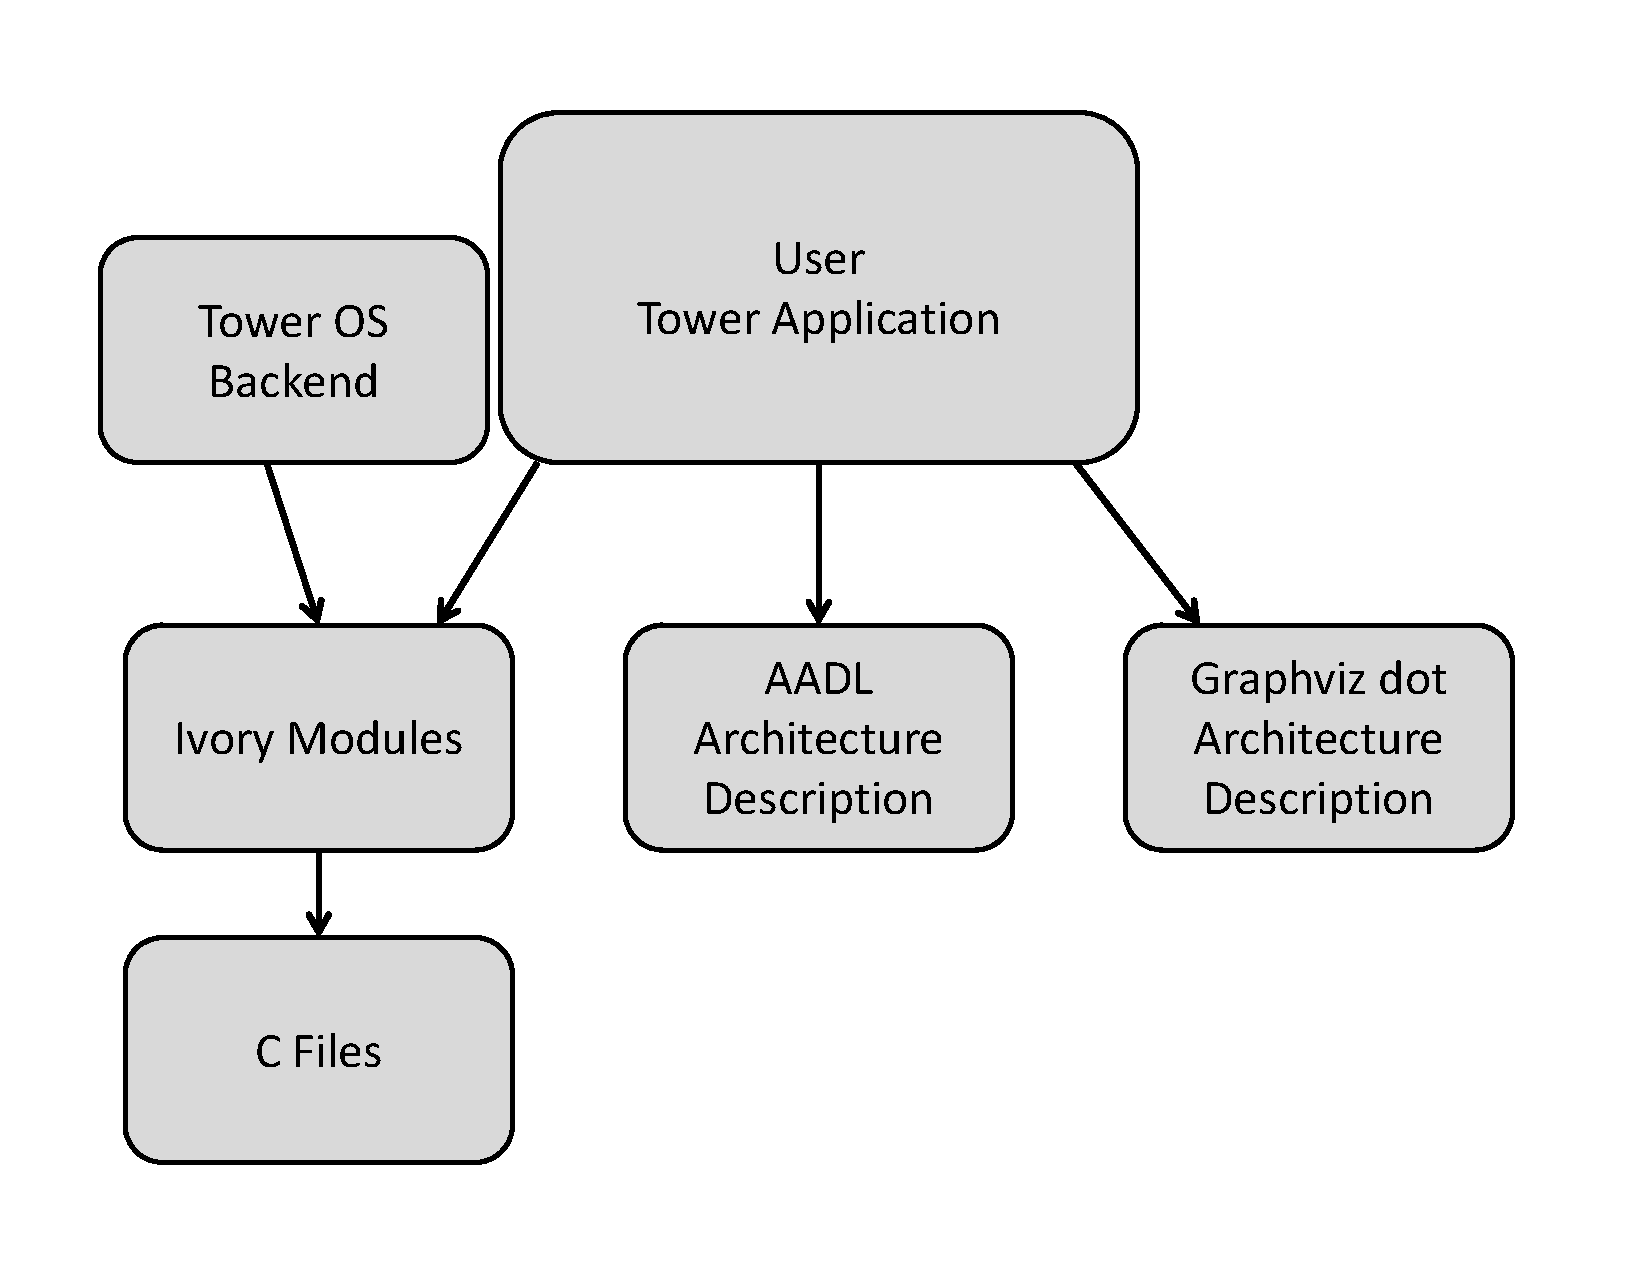
\includegraphics[width=6cm]{figures/tower-artifacts-dia}
%%   \end{center}
%%   \caption[Tower artifacts]{Tower artifact generation.}
%% \label{fig:towerArtifacts}
%% \end{figure}

In the Tower frontend, the programmer specifies a system that can be compiled into
multiple artifacts.

Tower is designed to support different operating systems via a swappable
backend. Since all code that touches operating system primitives is generated by
Tower, it is trivial for the user to specify a system and compile it for
different operating systems. Tower supports both the open-soure
FreeRTOS\cite{freertos} as well as the formally-verified
eChronos RTOS\cite{echronos} development by NICTA.

%% The static tower graph of channels and tasks also makes it possible to
%% describe the system architecture to external tools. 

Tower has a backend which generates a system description in the Architecture
Analysis and Design Language (AADL)~\cite{SAE:AADL}. We also built a backend for
the Graphviz dot language.  These output formats make it possible to visualize,
analyze, and automatically check properties about the system.  %% This is an
%% important feature when working with teams that may not all be literate in
%% Ivory/Tower.

We were pleased by the productivity improvements and correctness guarantees the
Tower language provided. In all, it took about 4 engineer-months to build Tower,
and a total of about 3000 lines of Haskell code.

\paragraph{Tower example}
In Figure~\ref{fig:tower-ex}, we sketch a small Tower example that is
representative of a device driver that blinks an LED at the rate of 100 ticks
(the duration of a tick is dependent on the RTOS backend to Tower used.)  Small
simplifications to Tower have been made in the code, eliding details relating to
code generation and backend selection.

In the third column the program, defined in the \cd{Tower} monad, initializes a
channel between two tasks as well as the tasks themselves.  A channel, or queue,
consists of a transmit (\cd{tx}) and receive (\cd{rx}) endpoints, respectively.
The \cd{blink} task is an RTOS task that will send output to the
\cd{lightswitch} task, which toggles the LED based on the incoming Boolean
values.

The \cd{blink} task is defined in column three.  It takes a channel source and
returns a program in the \cd{Task} monad.  The task initializes first
initializes an emitter for the channel then creates a reference to private but
globally-allocated memory.  Every 100 ticks, an Ivory action is taken.  In this
case, the action is to make call an Ivory function, the one described in the
previous section, that toggles that value pointed to by \cd{res}.  This value
pointed to by \cd{res} is then emitted on the channel.

%%  controls
%% the LED.  The \cd{lightswitch} task toggles the 

%% application \cd{} has three statements in the \cd{Tower} monad.
%% \cd{channel} gives a fresh \cd{Channel}. \cd{task "blink"} instantiates a task
%% defined by \cd{blink}, operating on the channel just created. \cd{task
%% "lightswitch"} defines another task with an event handler that takes the value
%% of the message recieved on the channel, and performs an action depending on
%% whether the boolean was true or false. Definitions for \cd{turnOn},
%% \cd{turnOff}, and \cd{light} are elided.


%% In the
%% example, we define a function \cd{blink} that takes a \cd{Channel (Stored
%%   IBool)} - that is, a Tower communication channel which contains messages of
%% booleans. The definition of \cd{blink} has two statements in the \cd{Task}
%% monad. \cd{withChannelEmitter chan} creates an \cd{Emitter (Stored IBool)} from
%% the \cd{Channel}, bringing that emmitter into scope for the particular task. The
%% second action, `onPeriod`, takes a period (in milliseconds) and an event handler
%% of type \cd{Uint32 -> Ivory eff ()}.

%% The definition of \cd{body}, the handler for the periodic event declared in
%% \cd{blink}, produces a fragment of Ivory code. The macro \cd{emit\_ tx} has type
%% \cd{IBool -> Ivory eff ()}. Its argument, \cd{even currTime}, calculates whether
%% the current time, modulo the period, is even or odd. We must make an \cd{Uint32}
%% - Ivory's 32-bit signed integer type - out of \cd{period :: Integer}, with
%% \cd{fromIntegral}.





\section{SMACCMPilot: a High-Assurance Autopilot}
\label{sec:smaccmpilot}

\begin{figure}[ht!]
  \begin{center}
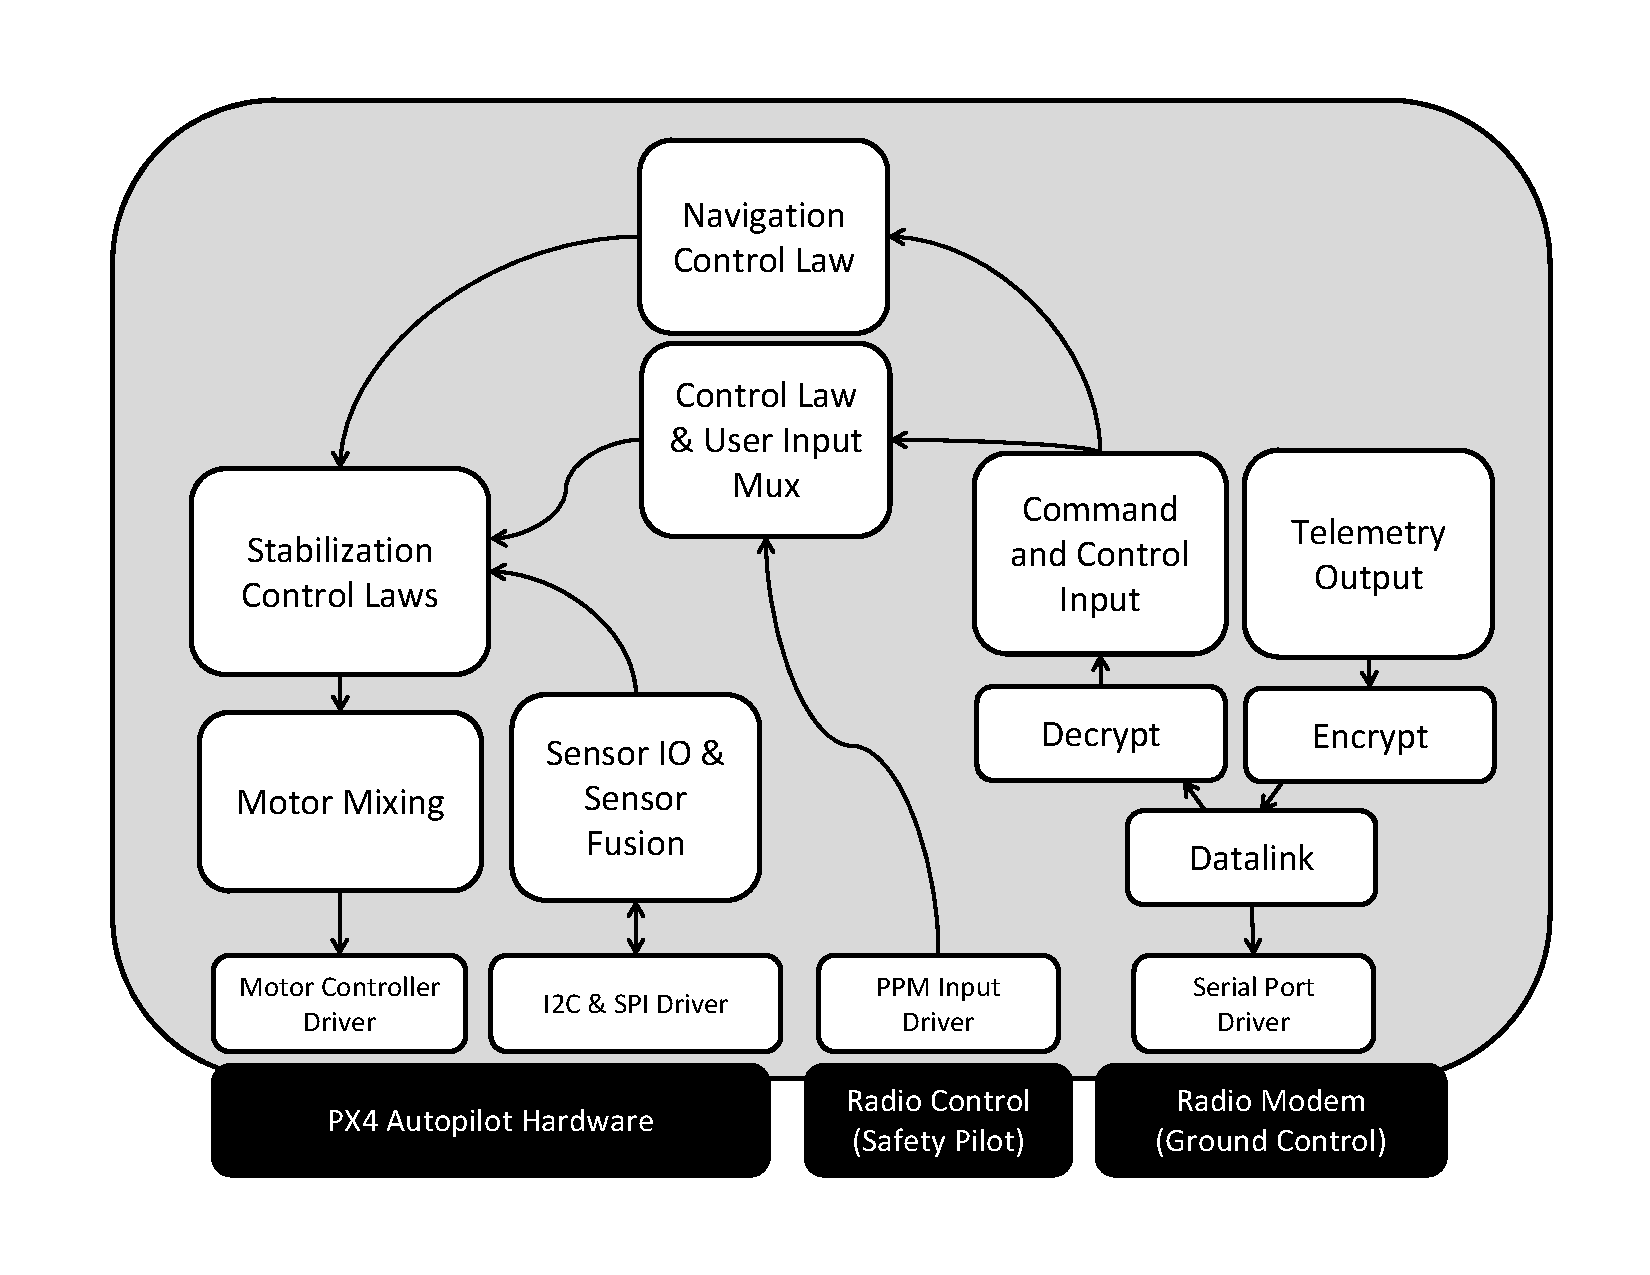
\includegraphics[width=8cm]{figures/smaccmpilot-diagram-jan14}
  \end{center}
\caption[SMACCMPilot software architecture]{
Simplified diagram of SMACCMPilot
software architecture. Tasks written in Ivory are shown as white boxes,
tasks implemented in legacy C++ code are gray boxes,
channels are arrows,
hardware components are black boxes.}
\label{fig:smaccmpilotSwArch}
\end{figure}

Our goal was to build a robust autopilot. The result is
SMACCMPilot, an open-source (BSD Licensed) autopilot system for quadcopter
unmanned air vehicles (UAVs).
It is complete embedded system implemented with
the Ivory/Tower tools.
It includes low-level IO peripheral drivers, an encrypted
communication protocol stack, and several layers of control systems.

SMACCMPilot runs on open source flight controller hardware from the PX4
Autopilot project~\cite{px4-proj}. The hardware platform is
a custom printed circuit board with an ARM Cortex M4 microcontroller and the
accelerometer, magnetometer, gyroscope, and barometer sensors used to
determine the orientation and altitude of the vehicle.

A simplified software architecture of SMACCMPilot is shown in
Figure~\ref{fig:smaccmpilotSwArch}.
The flight control software is primarily responsible for reading the sensors,
estimating the vehicle's attitude and position using sensor fusion, calculating
control outputs, and sending motor power commands to the motor controllers.
Higher level control loops manage navigation, and an encrypted command, control,
and telemetry link interprets ground station instructions, sends system state to
the operator, and permits online tuning of control loop parameters.

The result is a reasonably complex piece of embedded software. SMACCMPilot has
30 tasks connected by 47 channels, and 57 globally shared state variables. Most
of those shared state variables are control loop tuning parameters, which can be
modified by commands sent over the telemetry link.

SMACCMPilot was developed alongside the Ivory/Tower tools.  The complete system
took approximately 22 engineer-months to develop.  The low level drivers for the
system were written first in C, then transliterated to Ivory as the language
became mature enough to support them. We built a stack for command, control, and
telemetry, encapsulated in an encrypted packet protocol. A few components from
the ArduPilot open source project, the biggest of which is a 10kloc C++ library
for inertial sensor fusion, are still used inside SMACCMPilot.

\paragraph{Complexity comparison}
The SMACCMPilot application code is 10kloc of Ivory, the board support code
is 3kloc of Ivory, and the telemetry link binary packing and unpacking
code is a machine generated 10kloc of Ivory code. When compiled, the complete
application
is 48kloc of generated C~code, and depends on some external C libraries to
implement the operating system (4kloc) and other functions, such as sensor
fusion.  This compares favorably to existing open source flight controller
systems.

We can compare this to two systems which have a similar feature set and run on
similar hardware to SMACCMPilot.  The ArduPilot project~\cite{apm-proj} and the
PX4 project are popular open source autopilots, both of which have more high
level navagation and autonomy capabilities than SMACCMPilot.  Both implement all
of the low level drivers to support similar (or identical) microcontroller based
flight controller boards, comparable control laws, and implement the same
MAVLink telemetry protocol.

The ArduPilot project is over 60kloc of C++, runs in three pseudo-threads, and
supports at least four distinct autopilot hardware platforms. The PX4 Autopilot
software stack has 25kloc of C/C++ application code, 25kloc of C/C++ platform
support code, and depends on the large (50kloc+) NuttX operating system.



\section{The Good}

In this section, we discuss some of the benefits of EDSLs for embedded
programming.  Some of these benefits were surprising to us, even with our
previous experience in functional programming and embedded development.

\paragraph{Type-checking as interpretation}
Build times are non-trivial for large software systems.  (Some of our kernel
developers at Galois are known to have novels on hand to read during the build
and test cycle.)  Modern C compilers are reasonably fast, but compiling 10s of
thousands of lines of code can take 10s of seconds.  In addition, during testing
and integration, our build includes various test builds and builds for multiple
operating-system and hardware configurations meaning that the same source code
gets recompiled multiple times.

Then, to execute the software on the embedded device, we have to write the
software to the device's memory (we refer to this as ``flashing'' the device,
since the executable is stored in non-volatile flash memory on a number of
microcontrollers).  Flashing can take many seconds.

All this is to say that the time between making a change in the sources to when
the changes are tested can be many seconds or minutes.  The situation is
exacerbated when we use an EDSL to generate the C code; the EDSL must be
compiled by Haskell; the haskell program is executed to generate the C code, and
then the C code is compiled, linked, and flashed.

High-level languages like Haskell have a read-eval-print-loop (REPL),
significantly reducing development time since it allows the developer to
type-check and test programs without going through the full compilation cycle.
Embedded C does not have a REPL, and building one is a major undertaking: it
would require a model of the sensors and devices the program interacts with, a
model of the operating system, as well as library code (e.g.,
glibc).\footnote{An emulator like QEMU~\cite{} does not solve the problem: (1)
  QEMU is not an interpreter, and often it is not useful at all if the
  application code interacts with sensors and external devices.}



\paragraph{Mario programming}
We are all just plumbers.

\paragraph{The five-minute driver}
Safe drivers as easy as user-code.  (Note Microsoft focus on drivers)

\lp{no seg faults}




\section{The Bad}


\begin{compactitem}
\item type-checking errors, compile-cycle (Haskell + C). 
\item Tracking file/line no. from C to haskell.
\item Code duplication.
\item macro-expansion (i.e., memory addresses).
\item cabal with make
\end{compactitem}

template haskell: make another level above the haskell type-checking



\section{Conclusion}

\todo{talk about assurance/productivity trade-offs}



%% \appendix
%% \section{Appendix Title}



\acks

This work is supported by DARPA under contract \lp{contract
  no. FA8750-12-9-0169}.  Opinions expressed herein are our own.  A number of
people have provided input and adivce; we particularly thank Kathleen Fisher,
Iavor Diatchki, and Andrew Tridgell.

% We recommend abbrvnat bibliography style.

\bibliographystyle{abbrvnat}
\bibliography{paper}

% The bibliography should be embedded for final submission.

%% \begin{thebibliography}{}
%% \softraggedright

%% \bibitem[Smith et~al.(2009)Smith, Jones]{smith02}
%% P. Q. Smith, and X. Y. Jones. ...reference text...

%% \end{thebibliography}


\end{document}

%                       Revision History
%                       -------- -------
%  Date         Person  Ver.    Change
%  ----         ------  ----    ------

%  2013.06.29   TU      0.1--4  comments on permission/copyright notices

